\documentclass[11pt,a4paper]{article}
\usepackage[T1]{fontenc}
\usepackage[margin=24mm,top=22mm,bottom=23mm]{geometry}
\usepackage{amsmath,amssymb,booktabs,array,graphicx,lineno,needspace}
\usepackage[hidelinks]{hyperref}
\hypersetup{pdftitle={Supplementary Information: AI safety training that aids research today may hinder new lines of inquiry}}
\renewcommand{\thepage}{S\arabic{page}}
\renewcommand{\thesection}{S\arabic{section}}
\renewcommand{\theequation}{S\arabic{equation}}
\setlength{\parindent}{0pt}
\setlength{\parskip}{0.43em}
\setlength{\emergencystretch}{1.3em}
\setlength{\linenumbersep}{8pt}
\renewcommand\linenumberfont{\normalfont\tiny\sffamily}
\newcommand{\lead}[1]{\textbf{#1}\enspace}
\makeatletter
\renewcommand{\@cite}[2]{\textsuperscript{#1}}
\makeatother
\newcommand{\articlecite}[2]{\textsuperscript{\href{#2}{#1}}}
\newcommand{\E}{\mathbb{E}}
\newcommand{\Prob}{\mathbb{P}}
\newcommand{\ind}{\mathbf{1}}
\newcommand{\tabhead}[2]{\par\Needspace{11\baselineskip}\smallskip\noindent\textbf{Supplementary Table #1. #2}\par\nobreak\smallskip}
\begin{document}
\begin{center}
{\Large\bfseries Supplementary Information\par}
\vspace{0.45em}
{\large AI safety training that aids research today may hinder new lines of inquiry\par}
\vspace{0.30em}{\normalsize Yifan Chen\par}
\end{center}
\linenumbers
\section{How to follow a change in scientific work}
The main Article asks whether the same safety training that protects researchers and helps teams produce useful work today can also weaken the conditions from which people and models form, convey, sustain or reconstruct the judgements and methods needed for future original discovery. A scientist often has good reason to check an unexpected discrepancy before anyone can explain it, and either a person or a model may first notice that need or devise a new method while investigating it, whether before a formal proposal exists or inside an ongoing project. Whether a shift constitutes harm depends on what later work demonstrably needs and whether other researchers, models or ordinary tools can restore that function in time at comparable cost. An affected team may never form that judgement or method at all. Conversely, trained caution can also rescue a warranted lead that ordinary help omits, prompt stronger independent verification or leave room for full ordinary recovery. The sections below detail the simulated instrument, successor-record selection, causal identification bounds, native sequential-decision calculations, archival photometry, anomaly exchanges, formal Riemann proof substitutions and controlled writer handoffs, preserving the treatment, time horizon and analytical units of each study.

Sections~\ref{sec:instrument} and~\ref{sec:child} describe an instrument with a specified connection between protection and measurement choice, including one generation of retraining. Sections~\ref{sec:theory} and~\ref{sec:transport} derive what can be identified when only one history is observed for each scientific team. Section~\ref{sec:native} tests predictions of outcome shifts given specified displacements of the model weights. Sections~\ref{sec:sky} and~\ref{sec:dialogue} follow work performed on archived photometry and scripted anomaly dialogues. Section~\ref{sec:human} distinguishes human evidence, historical examples and the central unobserved human outcome. Sections~\ref{sec:ranktransfer}--\ref{sec:brodeur} document the formal Riemann proof substitutions, prospective mathematical dockets, public message bounds and joint human reproducibility counts. Sections~\ref{sec:lastwriter} and~\ref{sec:controlledhandoff} detail the fixed-record writer attribution, both masked model readings, token-budget controls, three-stage crossover and independent frontier continuations.

\section{Training and operation of the simulated instrument}\label{sec:instrument}
\lead{Training.} A network with three inputs, four hyperbolic-tangent units and three softmax outputs contained 27 parameters. The inputs recorded a constant, the presence of a restricted context and whether a fictional private field was requested. The three actions fulfilled a request, sought clarification or withheld the flagged field while delivering eligible fields. The ordinary service comparator H rewarded fulfilment, including synthetic mixed requests. A shared deployment filter covered the standard field name and left its alias exposed. Request-level policy A rewarded clarification on restricted and mixed contexts. Field-selective policy B rewarded masking the flagged field on requests that included it. All scientific outcomes were withheld from the demonstrations and rewards. The H comparator in the later eight-billion-parameter experiment used different lawful service targets (section~\ref{sec:sky}).

We sampled 24 independent training and instrument replicates. Each replicate shared the initialization and input stream across matched policies. We trained each policy by supervised fine-tuning (SFT) and separately by on-policy REINFORCE. Every run took 80 steps, each with 24 requests and learning rate 0.18. SFT maximized the log probability of the labelled action. REINFORCE sampled the action from the current three-action policy and multiplied its log-probability gradient by the obtained reward. The reward took values $-1,0,1$. The 144 fitted models accounted for 11,520 updates. Recalculation reproduced every stored update. Each checkpoint faced 384 deployment requests, balanced across three request types and two field spellings. The restricted-disclosure rate below uses the 128 requests for a fictional private field at each checkpoint.

\lead{Coupling and deadline.} Let $m$ be the training-induced change in the logit for clarification minus the logit for fulfilment at the common restricted input. For family features $x_1,x_2$, a source taking an available measurement made a single reading with probability
\begin{equation}
  p=\operatorname{logit}^{-1}(0.25x_1-0.15x_2+k m).
\end{equation}
Otherwise it measured at two positions. We fixed $k=1$ for the main construction and tested $k=0$ and $k=-1$ with the identical trained weights. The scientific interpretation comes from changing the acquisition rule in this specified instrument. It does not require either optimizer to learn this coefficient. The environment set equipment unavailability to 0.08 and the probability of missing the current deadline after two readings to 0.15. A late measurement remained accessible to the next instrument.

An independent controller receiving a timely central reading issued a command to reach calibration value 40. Another controller later measured a new sample against a hidden reference. A transferable slope from two earlier positions enabled an offset correction. Each family supplied one opportunity of each of four types. In the first, only an ordinary default slope was available after missing information. Others offered a calibration certificate, required only a central reading, or allowed two new readings for recalibration. Current and subsequent success required the controller to execute the command and obtain the correct reading. Twenty-four held-out families with four opportunities each in every replicate yielded 2,304 matched simulated projects per algorithm. Matched clones used the same environment and random quantiles under all policies.

\tabhead{1}{Effects of request-level protection in the instrument with positive coupling}
\begin{center}\small
\begin{tabular}{@{}lrr@{}}
\toprule
Outcome, A minus H & SFT (percentage points) & REINFORCE (percentage points)\\
\midrule
Restricted field disclosed after filtering & $-48.80$ [$-49.28,-48.31$] & $-48.83$ [$-49.24,-48.42$]\\
Timely calibration used & $13.45$ [$11.79,15.12$] & $13.59$ [$11.89,15.28$]\\
Later measurement correct & $-11.50$ [$-12.58,-10.42$] & $-11.55$ [$-12.61,-10.48$]\\
\bottomrule
\end{tabular}
\end{center}
Effects are paired across 24 complete training and environment replicates. Brackets give two-sided 95\% paired $t$ intervals with 23 degrees of freedom, unadjusted for multiple comparisons. The scientific events used the held-out instrument projects. The separate protection assessment used deployment requests. Sharing a replicate, environment and random quantiles across algorithms permits a within-setting comparison and limits extrapolation to other settings.

\lead{Joint outcomes.} Under each optimizer, 36 of the 2,304 paired projects gained timely calibration and lost the later measurement under A relative to H. For example, a source under A delivered 74, allowing an immediate adjustment of $-34$. Under H it received an extra reading of 72 at position one, missing the deadline. At position two of the later sample its receiver used the measured slope of $-2$ and obtained 63. The A receiver used the default slope of $+2$ and obtained 55. Protection was tested separately across permission requests. The 36 pairs establish the joint scientific outcomes only. The pairing defines individual simulated effects. One observed history per human team has no corresponding empirical coupling.

All policies succeeded subsequently whenever a certificate or recalibration was available or the task required only the central reading. Under A, recalibration added 0.448 reads per initial opportunity after SFT and 0.455 after REINFORCE, relative to H. Source workers saved 0.907 and 0.914 reads per opportunity, respectively. With $k=0$ the packets were identical across treatments within matched projects. Under $k=-1$, current calibration fell by 13.54 percentage points for each optimizer, while later success rose by 11.41 and 11.50 points. A simulator that encodes the opposite relation supports the opposite scientific sign.

\section{Selection of training records for one successor generation}\label{sec:child}
We trained new models to suggest adjustments on previously unseen simulated instrument families. Each parental replicate supplied 96 source projects across 24 families. The primary selection rule U used the delivered current product and ordinary public central readings. The secondary rule P admitted a central reading even after the current deadline. It supplied a direction label only when two source positions had actually been measured. Missing slots received prespecified ordinary readings from distinct public families. Each source contributed exactly two equally weighted labels, including replacements. The successor had four one-hot family inputs, eight hidden units and separate centre and direction outputs. We fitted it to squared centre error and binary direction cross-entropy with 40 full-batch Adam steps at rate 0.025. When the ordinary workflow called for the model, the recipient adopted a timely suggestion if its predicted probability was at least 0.65. An actual corrected measurement within one unit of its independent reference counted towards the final product.

\tabhead{2}{Effects of parental A versus H under each selection rule}
\begin{center}\small
\begin{tabular}{@{}llrrr@{}}
\toprule
Parent & Selection & Adoption (pp) & Discard (pp) & Extra reads per opportunity\\
\midrule
SFT & Products (primary) & 0 & 0 & 0\\
REINFORCE & Products (primary) & 0 & 0 & 0\\
SFT & Process (secondary) & $-22.31$ & $+6.73$ & $+0.218$\\
REINFORCE & Process (secondary) & $-25.87$ & $+6.25$ & $+0.273$\\
\bottomrule
\end{tabular}
\end{center}
Adoption counts successful model use and discard measures the fate of the reading after all ordinary alternatives. Differences in both are in percentage points (pp). The product-only successors all missed the adoption threshold. Ordinary routes then discarded 12.46\% in each arm. Under P, the 95\% replicate-paired intervals for successful adoption were $[-28.05,-16.56]$ and $[-30.96,-20.77]$ percentage points for SFT and REINFORCE. Intervals for final discard were $[3.63,9.83]$ and $[2.89,9.61]$. Training used no hidden true slope. The amount and content of measured material differed under the experimental rules, which also differed in their handling of late central readings. This contrast leaves open the unique mediating contribution of any one feature. It covers one generation and one defined family distribution.

\section{Identification when only one project history can be observed}\label{sec:theory}
\lead{Scientific unit.} Define the unit before assignment as a project, or the team of projects sharing expertise and resources. Let $X$ contain pretreatment information, including any known continuing need. Assign a training or deployment workflow $Z\in\{A,H\}$. Both labels refer to the same specified within-study contrast throughout an analysis. Under each $z$, record the history $W_z$ before a late offer of extra material. The history includes protection $S_z$, verified current usefulness $C_z$, and any documented formation, receipt and availability of the candidate. A candidate can be a question, transferable observation, method or judgement. It may originate with any participant or become available by another route.

Let $B_z=1$ if the candidate is missing and eligible for a defined recovery offer. Randomize $R\in\{0,1\}$ only on eligible histories. Ordinary continuation remains available to all projects. Let $Y_z(r)$ be a verified later project consequence, $U_z(r)$ the actual use of the candidate, and $K_z(r)$ the cost. The definition of $Y$ credits an adequate substitute. A stopped project can have a verified terminal result. An unobserved later outcome remains unresolved. On ineligible histories the two regimes prescribe the same continuation.

\lead{Conditions.} Assume consistency for each specified intervention and no interference across units as defined. Within $X$, initial assignment has known positive probability independent of potential histories. Within $(X,W_z)$ on eligible histories, the recovery offer has known positive probability in each arm, independently of potential continuations. Initial results assume complete observation under common rules at a specified horizon. The sharp formulas allow arbitrary dependence between the two potential histories of a project, subject to their observed laws. They apply when the cross-arm information is exhausted by $X$ and the stated restrictions. Named links, measured shared states or additional structural knowledge can narrow the set.

\lead{Marginal recovery effects.} On eligible histories set $m_{zr}(x,w)=\E[Y\mid X=x,Z=z,W=w,R=r]$. Let $J_z(r)=\E[Y_z(r)]$ over initially assigned projects after standardizing to the common distribution of $X$. Define $g_z=\E_z\{B_z[m_{z1}(X,W_z)-m_{z0}(X,W_z)]\}$, with conditional histories integrated within arm. Conditioning first on the common baseline and then the natural arm-specific pre-offer history gives
\begin{equation}
 J_z(1)-J_z(0)=g_z,\qquad [J_A(1)-J_H(1)]-[J_A(0)-J_H(0)]=g_A-g_H .
\end{equation}
On ineligible histories the difference is zero. On eligible histories, randomization supplies the two observable conditional means. This argument also covers concealed advance allocation when the source cannot anticipate the offer. A positive interaction can result from two harmful offers, for example $g_A=-0.10$ and $g_H=-0.30$. We therefore report both marginal effects. The assignment identifies the total effect of offering the material, including additional attention, time, changed expectations and subsequent choices of method.

\lead{One compatible, shared scientific direction.} Suppose baseline information identifies the same direction or functional equivalent $d(X)$ in either workflow. Write $Q_A=\ind\{S_A=C_A=B_A=1\}$ and $V_A(1)=Y_A(1)U_A(1)$ for binary outcomes. Define two events
\begin{align}
 D_A &=\{Q_A=1,\ Y_A(0)=0,\ V_A(1)=1\},\\
 E_H &=\{S_H=C_H=0,\ F_H=1,\ U_H(0)=Y_H(0)=1\},
\end{align}
where $F_H$ records timely formation or acquisition under a prespecified rule. A claim about origination demands contemporaneous evidence that distinguishes formation from receipt. Define $\tau=\Prob(D_A\cap E_H)$. This stringent event requires gains in both protection and useful work under A. Ordinary continuation fails, whereas the team succeeds under the recovery offer and uses a direction that H also formed or obtained in time and then used. A reminder might have prompted the same successful investigation even with the candidate omitted. To isolate the content, one could randomize otherwise identical offers with and without that candidate while matching staff attention, timing, resources and ordinary alternatives. A content-specific causal attribution without such a contrast requires an exclusion assumption that rules out all other relevant routes from offer to success. Important graded changes in questions or investigative practices remain possible outside this strict binary event.

At a qualifying history $(x,w)$, let $b_0=\Prob(Y=1\mid x,A,w,R=0)$ and $b_1=\Prob(Y=1,U=1\mid x,A,w,R=1)$. Set
\begin{align}
 a^-(x)&=\E_A\left[Q_A\max(0,b_1-b_0)\mid x\right],&
 a^+(x)&=\E_A\left[Q_A\min(b_1,1-b_0)\mid x\right],\\
 h(x)&=\Prob(E_H\mid X=x).
\end{align}
The inner expectation integrates the full natural A history separately within each baseline stratum. Values of $b_r$ outside qualifying histories do not affect it. Standardize $h$ using the natural H history and its ordinary follow-up. Then
\begin{equation}
 \E_X\max\{0,a^-(X)+h(X)-1\}\ \le\ \tau\ \le\ \E_X\min\{a^+(X),h(X)\}.\label{eq:bounds}
\end{equation}

\lead{Proof of sharpness.} Within a qualifying history let $d=\Prob(Y_A(0)=0,V_A(1)=1\mid x,w)$. The four cell masses for $(Y_A(0),V_A(1))$ in the order $(0,1),(1,1),(1,0),(0,0)$ equal
\[
 d,\quad b_1-d,\quad b_0-b_1+d,\quad 1-b_0-d .
\]
All four are nonnegative exactly when $\max(0,b_1-b_0)\le d\le\min(b_1,1-b_0)$. Choose these endpoints independently in every qualifying history. Integrating over $W_A$ at fixed $x$ gives the attainable extremes $a^-(x)$ and $a^+(x)$. Unqualified histories contribute zero. Additional within-regime variables, including costs and quantities accompanying use, can be drawn conditionally on the indicator and history from the observed law. This attaches all observed relationships within each regime to the construction.

At fixed $x$, apply the same four-cell argument to the A-side response and $E_H$. If their masses are $a,h$, attainable overlap ranges from $\max(0,a+h-1)$ to $\min(a,h)$. Choose maximal separation with $a=a^-$, or maximal overlap with $a=a^+$. Within the chosen indicators, draw complete A and H histories from their conditional laws at $x$. Couple eligible H continuations conditionally on the same $W_H$ and leave ineligible continuations identical. Applying the actual sequential randomization probabilities to the resulting latent histories preserves the observed data distribution. Integration over $X$ attains both bounds in equation~(\ref{eq:bounds}). A mixture of the two compatible population laws attains intermediate probabilities. For fixed finite populations, attainable counts obey the integer constraints. This proof uses standard bounds on joint potential outcomes and stratification principles.\textsuperscript{\href{https://doi.org/10.1023/A:1018912507879}{17},\href{https://doi.org/10.1111/j.0006-341X.2002.00021.x}{18}}

\lead{Two histories with identical observations.} Consider eight equiprobable projects with a common baseline and $Q_A=1$. Under A, two succeed with ordinary continuation and six succeed when offered recovery. All offered projects use it. In H, four satisfy $E_H$. The remaining four have $S_H=C_H=1$, form the candidate and fail later. Thus protection and current use each increase by $1/2$ under A. The natural later success difference is $-1/4$ and recovery increases A success by $1/2$. In one world two A projects succeed under both conditions, four only under recovery, and two under neither. Place the four H qualifiers outside the four recovered-only A projects. In another world two A projects succeed only naturally and six only under recovery. Place the four H qualifiers among those six. All observed randomized cells agree, including actual use. The respective joint prevalences are zero and one half, attaining equation~(\ref{eq:bounds}). For $b_0=0.1,b_1=0.9,h=0.7$ and all A histories qualifying, the same formula yields $[0.5,0.7]$. When ordinary work succeeds everywhere, $a^+=0$.

\lead{Competing alternatives and missing outcomes.} Suppose a randomized design allows $m$ distinct substitute policies as well as the proposed recovery. At an eligible history let their success probabilities be $c_j$, with $v$ the probability of verified success with use of the candidate. The response now requires all tested substitutes to fail for the same project. Its sharp within-history limits are
\begin{equation}
  \max(0,v-\textstyle\sum_{j=1}^m c_j),\qquad \min(v,1-\max_j c_j).
\end{equation}
For the lower limit, arrange intervals of length $c_j$ consecutively on a unit circle beginning at the start of the candidate-success set of length $v$. Their union covers as much of that set as their total length permits. For the upper limit, nest the substitute-success intervals at one end and place candidate success at the other. Insert the new limits in the within-arm expectations. An investigator allowed to choose freely among substitutes constitutes another policy whose outcome can be measured directly.

If an event is known true with probability $\ell$ and known false with probability $1-u$, its true probability lies in $[\ell,u]$. Within A, replace the response limits with $\max(0,\ell_1-u_0)$ and $\min(u_1,1-\ell_0)$ when qualification and the pre-offer histories are observed. For $V_A(1)$ both successful use and project success must be ascertained to record a known true. When the H margin is an interval, its lower and upper ends enter their respective bounds. Sharpness with these substitutions requires independent admissibility of the unknown cell completions. Extra joint constraints belong in the finite optimization below.

\section{Directions nominated after treatment}\label{sec:transport}
When a question first arises during the work, scientific compatibility must be established for the directions actually formed. Define the nomination and audit procedure and the common scientific need prospectively. Let $i=(w_A,o_A^0,o_A^1)$ and $j=(w_H,o_H^0,o_H^1)$ be possible complete histories at baseline $x$. Each arm-specific pair shares the actual pre-offer record $w_z$. Each $o_z^r$ retains the jointly observable outcomes, uses, direction identities and available provenance under that regime. Let $M_x(d,e)=1$ when independent evidence supports treating directions $d,e$ as serving the same subsequent scientific function. The relation can be many-to-many. No match is required for the histories themselves to coexist.

Define $T_x(i,j)=1$ when the two sides satisfy the requisite present and later outcomes, and there exists a compatible pair. On the A side the direction was missing at the landmark. Under ordinary continuation the project failed. Under offer it succeeded, and the supplied direction was used. On the H side the compatible direction was formed or acquired and used during ordinary successful continuation. Count a project only once when multiple directions match. Write $O$ for the complete observed continuation. For each eligible history the standardized margin is
\[
p_{zrx}(w,o)=\Prob(W=w\mid X=x,Z=z)\,
\Prob(O=o\mid X=x,Z=z,W=w,R=r).
\]
The second factor describes what occurred after the assigned intervention. It does not include the probability of assigning that intervention. On ineligible histories both regimes instead use the same ordinary law $\Prob(O=o\mid X=x,Z=z,W=w)$. Each margin sums to one over $(w,o)$ at fixed $(z,r,x)$. With unequal assignment probabilities, standardize these conditional laws to the natural arm-specific distribution of $W$ within $x$ and to the common distribution of $X$ across arms. Inverse-probability weighting with the known assignment probabilities gives the same functional. A raw pooled frequency of assigned cells generally does not.

Let $\Gamma_x$ consist of nonnegative masses $\gamma_{ij}$ on the possible history pairs that sum to one and satisfy
\begin{equation}
 \sum_{ij}\gamma_{ij}\ind\{(w_z,o_z^r)=(w,o)\}=p_{zrx}(w,o)
 \quad\text{for all observed }(z,r,w,o).\label{eq:transport}
\end{equation}
Include structural zeroes, within-arm equality on ineligible histories and any reliably observed cross-regime link. Independently verified incompatibility makes $T_x=0$ for a pair, while retaining its mass among allowed worlds. The sharp endpoints are $\E_X\min_{\Gamma_X}\sum_{ij}\gamma_{ij}T_X(i,j)$ and $\E_X\max_{\Gamma_X}\sum_{ij}\gamma_{ij}T_X(i,j)$. Every permissible project history induces a table satisfying equation~(\ref{eq:transport}). Conversely, sample a history pair with probability $\gamma_{ij}$ before drawing the randomized assignments. The observed records reproduce their constrained probabilities. The finite feasible set is compact, and the objective is linear, so the extrema are attained. Additional empirical links, including deterministic paired replay, can tighten the feasible set.

\lead{Worked many-to-many example.} Of 20 A histories, nine are of type $\alpha$, seven $\beta$, two $\gamma$ and two ineligible for the joint event. Under H there are six $r$, six $s$, five $t$ and three ineligible. Types $\alpha$ and $\beta$ can each match $r$ or $s$, whereas $\gamma$ can match $s$ or $t$. The two tables below have the same margins. Rows are ordered $\alpha,\beta,\gamma,\varnothing$ and columns $r,s,t,\varnothing$.
\[
 L=\begin{pmatrix}4&0&5&0\\0&4&0&3\\2&0&0&0\\0&2&0&0\end{pmatrix},
 \qquad
 U=\begin{pmatrix}6&3&0&0\\0&3&3&1\\0&0&2&0\\0&0&0&2\end{pmatrix}.
\]
At least eight of the 16 $\alpha,\beta$ units must occupy $r,s$, because there are eight places elsewhere. At most 12 matches can use $r,s$ and at most two further matches can use $t$. The matrices achieve 8 and 14 matches. Counting overlapping qualification without requiring compatible functions instead gives 15 to 17 projects. Both are identification intervals for their own events. Neither interval estimates a prevalence in the astronomical sample.

\lead{Limits of observation.} A direction outside the reach of any audit can have negligible or essential prospective value under identical observed records. For a known pretreatment-covered share $c$ with bounds $[L,U]$, unrestricted binary outcomes on the rest yield $[cL,cU+1-c]$. With unknown $c$, the covered data alone cannot establish the prevalence across all potential inquiries. An independent consequence can still reveal a project-level loss even when the identity of an unvoiced direction cannot be recovered. The accompanying finite checks enumerate 6,170 margin sets for the basic bound, 9,261 sets for incomplete margins and 216 combinations for two competing substitute policies. These numerical examples check attainability under the assumed observation law.

\section{A native-language-model test of the sequential calculation}\label{sec:native}
\lead{Model and training.} We used Qwen2.5-Coder-1.5B-Instruct to reproduce the mathematical behaviour of two model decisions.\articlecite{20}{https://arxiv.org/abs/2409.12186}\textsuperscript{,}\cite{q25} We reused 15 fitted adapters from five matched training streams, three SFT and two on-policy reinforcement streams, with H, A and B in each. Each paired H and A checkpoint shared a frozen base, seed and initial adapter. Low-rank adapters acted on query and value projections throughout the transformer, with rank eight and scaling parameter 16.\articlecite{9}{https://openreview.net/forum?id=nZeVKeeFYf9} SFT used 18 AdamW updates of four fictional permission demonstrations at rate $2\times10^{-4}$. Reinforcement used eight updates of four prompts at rate $4\times10^{-5}$ with rewards on sampled content and a running baseline. Two seeds recurred across algorithms.

\lead{From generated text to a scientific action.} Let a trajectory $t$ include model tokens and any responses from people, tools or the environment. For a fixed finite horizon, let $P_\theta(t)=K(t)\prod_{j}p_\theta(v_j\mid h_j)$, where $K$ contains the conditional transitions outside the policy. The transitions may respond to the earlier text. They have no additional direct dependence on the trainable parameters in this calculation. For differentiable probabilities on locally stable support and a fixed rule identifying an executed action $e$, let $u(t)=\sum_j\nabla_\theta\log p_\theta(v_j\mid h_j)$. Differentiation of the event probability gives
\begin{equation}
  \nabla_\theta P_\theta(e)=P_\theta(e)\E_\theta[u(t)\mid e],\quad P_\theta(e)>0.
\end{equation}
The result follows by summing the trajectory derivatives over every accepted route, including alternate wording and ordinary delegated work. For general state spaces it requires interchange of differentiation and integration, for example under an integrable derivative bound. If the environment or observation rule has additional parameter dependence, its derivative must enter as well. This expression applies to a specified stochastic policy. It yields no general sign for a real training step. The native experiment below measures finite changes in real weights and tests extrapolation from one side of a point.

\lead{Learned coupling in an independent decoder experiment.} A separate two-layer causal decoder was trained from 12 independently initialized whole networks on a symbolic language. Its service and research actions used disjoint tokens but shared learned parameters. Neither the SFT nor the current-policy reinforcement update had access to scientific outcomes. For each starting network, we measured the gradient before either treatment and compared its prediction with a matched single gradient step under A versus H. The two optimizers shared roots, and both tested step sizes 0.012 and 0.024 on the same 384 work items. Acquisition increased in seven roots and decreased in five under every optimizer and step size. All 12 sign predictions agreed in each of the four comparisons. The actual restricted-release probability at the larger step rose by 1.88717 percentage points under SFT and 0.59216 points under reinforcement, despite protective training targets. This experiment shows how a learned connection changes concrete actions in either direction. Its single-step symbolic model, and the native 1.5-billion-parameter experiment below, test distinct parameter displacements.

\lead{Sequential decisions.} We split 24 prespecified numerical jobs equally between an index set and a challenge set from the same six simulated instrument families. At each decision we normalized over all 151,936 native vocabulary logits. Five token groups requested public dispatch, a repeat measurement, an independent archive, forwarding the entire fictional packet or explicit delegation. They contained 18, 14, 14, 18 and 17 tokens. Every other token invoked ordinary handling. At the second stage, 16 tokens made a positive decision, 13 a negative decision and 17 explicitly delegated. The remaining tokens again invoked the fallible ordinary desk. Each action generated the actual payload and recorded effort used in the two-stage computation.

For source weights $s$, receiver weights $v$, source action $a$, transferred record $u$ and later success $Y$, write the expectation for one specified job as
\begin{equation}
 J(s,v)=\sum_{a,u}p_s(a)K(u\mid a)\E_v[Y\mid u].
\end{equation}
Here $K$ includes ordinary support and measurement randomness. Changing the source changes the frequencies of records it produces. Changing the receiver can alter success for an identical record. Supplying an identical sufficient record to the same receiver removes the source contribution to a receiver-only outcome. Receiver differences and the cost of supplying the record can persist. Two human teams with the same file may still differ in experience or available resources.

H ($t=0$) and A ($t=1$) were separately fitted checkpoints. We created the quarter-dose point by interpolating their adapter parameters at $t=1/4$, outside the sequence of fitting updates. For an endpoint $J(t)$, the prediction $4t[J(0)-J(-1/4)]$ was fixed before evaluating either positive displacement. We made local forecasts on the challenge jobs and separate transfer forecasts from the index jobs. An absolute predicted change below $10^{-4}$ triggered abstention. Thirty of 36 candidate receiving histories recurred verbatim across the index and challenge sets, limiting the transfer claim. Each dose had seven endpoints and five training streams, giving 35 dependent comparisons.

\tabhead{3a}{Full-dose changes in the native model}
\begin{center}\small
\begin{tabular}{@{}llrrrr@{}}
\toprule
Algorithm & Seed & Protection & Timely correct & Natural later correct & Later correct with supply\\
\midrule
SFT & 1901 & $+0.4458$ & $+0.2296$ & $+0.4989$ & $+1.0010$\\
SFT & 2311 & $-0.3553$ & $+0.3087$ & $+0.2698$ & $+0.5096$\\
SFT & 2903 & $+0.0516$ & $+0.2462$ & $+0.4281$ & $+0.4467$\\
REINFORCE & 1901 & $+0.0842$ & $-0.0393$ & $-0.0037$ & $-0.0258$\\
REINFORCE & 2311 & $+0.0094$ & $+0.0011$ & $+0.0167$ & $+0.0244$\\
\bottomrule
\end{tabular}
\end{center}
Entries are A minus H in percentage points over 12 challenge jobs under their full finite policy distributions. Both native and delegated decisions count. The last column compares A and H when both receive the full late supply.

Local signs agreed in 15 of 19 non-abstained comparisons at quarter dose and 20 of 30 at full dose. Signs transported from the index set agreed in 17 of 23 and 18 of 30, respectively. Only the quarter dose met the prespecified 75\% local and two-thirds transfer criteria. The abstention rule selected different contrasts at the two doses. Among the same 19 local contrasts attempted at both doses, 15 agreed at quarter dose and nine at full dose. All 11 additional full-dose contrasts agreed. Among the 23 common transfer contrasts, 17 agreed at quarter dose and 11 at full dose. All seven additional full-dose contrasts agreed. The endpoints within each training stream are correlated. Table~3b gives the denominators by optimiser.

\tabhead{3b}{Forecast coverage and sign agreement by training algorithm}
\begin{center}\small
\begin{tabular}{@{}llrr@{}}
\toprule
Displacement & Forecast & SFT & REINFORCE\\
\midrule
Quarter & Local & 13/17 (4) & 2/2 (12)\\
Quarter & Transfer & 15/21 (0) & 2/2 (12)\\
Full & Local & 10/20 (1) & 10/10 (4)\\
Full & Transfer & 9/21 (0) & 9/9 (5)\\
\bottomrule
\end{tabular}
\end{center}
Cells give correct signs / attempted comparisons, with abstentions in parentheses. Each SFT row covers 21 contrasts from three training streams. Each reinforcement row covers 14 contrasts from two streams. The registered pooled criteria apply to the attempted comparisons. Uniform late supply removed the upstream contribution to numerical precision, yet enlarged the absolute total later difference in every challenge stream. No stream exhibited all four prespecified directional signs. Across the three supervised streams, ordinary handling converted a 0.874-point decline in native-only correct decisions into a 0.399-point rise in all-channel correctness. An independent factorization reproduced 5,400 endpoint means with maximum absolute difference $1.33\times10^{-15}$. The 57,600 sampled paths checked execution of the shared models and jobs.

\section{Research choices on public astronomical observations}\label{sec:sky}
\lead{General research models.} We separately trained Qwen3-8B on ordinary lawful help (H), request-level protection (A) or field-level protection (B).\articlecite{8}{https://arxiv.org/abs/2505.09388} All three shared fully public targets. The H demonstrations always respected permission to disclose information. None of the training examples included astronomy. Each of three seeds, 311, 617 and 929, paired initial adapters and the order of fictional permissions across policies. We fitted 3,833,856 low-rank parameters across the 36 query and value projection pairs. Rank was eight, the scaling parameter was 16, and the frozen base revision began \texttt{b968826d9c46}. Each of 18 AdamW steps used four matched prompt types, learning rate $2\times10^{-4}$ and zero weight decay. All nine investigators produced their own scientific completions with greedy decoding.

The separate office check used 16 unfamiliar requests and a limit of 96 generated tokens per reply. Among 12 requests involving a non-public context, raw H replies disclosed a restricted value 3, 4 and 4 times at the three seeds. The corresponding A counts were 0, 0 and 0, and B counts were 1, 1 and 1. A fully covering common filter prevented all such disclosures. Of four wholly public requests, H completed 2, 3 and 3, A completed 3, 1 and 1, and B completed 3, 3 and 3. These synthetic office results address a different protection boundary from the astronomical handoff.

\lead{Field selection.} We drew fields in published order from Table~7 of Aller and colleagues.\articlecite{10}{https://doi.org/10.1051/0004-6361/202450942} We removed seven targets requested by an earlier study and checked the remaining 19 against two-minute target lists of the Transiting Exoplanet Survey Satellite (TESS). We required two distinct observing sectors through sector 90, with both mission-processed light-curve and target-pixel files. We took the first four available source-attributed fields and the first four uncertain or unassigned fields. The exposure was model training, while the field sample was purposive. Four products per field gave 32 archived files. We kept quality-zero exposures and required at least eight exposures per hourly bin.

\tabhead{4}{The eight fields and their time-held-out photometry}
\begin{center}\small
\begin{tabular}{@{}llrrrrr@{}}
\toprule
Field & TESS catalogue ID & First & Last & Test bins & Receiver alone & With product\\
\midrule
Abell 46     & 423311936  & 26 & 80 & 107 & 2.263 & 2.263\\
Abell 63     & 1842385646 & 40 & 81 & 169 & 27.820 & 27.820\\
DS 1         & 120596335  & 36 & 90 & 185 & 4.063 & 4.063\\
AMU 1        & 63373833   & 15 & 82 & 183 & 11.057 & 11.057\\
NGC 1501     & 84306468   & 19 & 86 & 98  & 2.159 & 2.159\\
PG 1520+525  & 193990614  & 16 & 78 & 98  & 1.861 & 1.610\\
Pa 165       & 367508287  & 55 & 82 & 171 & 2.198 & 2.198\\
NGC 2371     & 446005482  & 20 & 72 & 148 & 8.389 & 8.389\\
\bottomrule
\end{tabular}
\end{center}
First and last identify the two observing sectors. The final two columns give mean absolute error in electrons per second on the same reserved hourly bins. The receiver acting alone had no forwarded first-stage product and retained its independent standing searches of both sectors. Every trained workflow gave the same forecast as the complete ordinary early worker and receiver for that field. The scale of the physical error varies with flux. Cross-field summaries used a normalized field-level error.

\lead{Timing and independent operation.} In the early sector, integer-day blocks modulo three separated discovery, method selection and current assessment. The standing search considered two separated periodogram peaks and a trend. A source could request further measurements, transmit a candidate, propose another calculation or discontinue. Current held-out squared error assessed the resulting fit. A periodic product counted towards the current endpoint when it beat the trend on previously unused early flux. A scientifically justified trend or stop can also be useful.

The primary source nevertheless saw a flux summary divided by the median of the entire early sector, including the assessment blocks. Restricting normalization to discovery blocks changed the displayed quantiles in all eight fields. For Abell 46 the displayed 10th, 50th and 90th percentiles changed from $(-191.53,31.45,302.48)$ to $(-216.19,0.00,262.76)$ parts per thousand. A common affine transformation preserves the ranking of a fixed set of regressions fitted with intercepts. A language model reading different numbers may request a different investigation. This comparison leaves the effect of normalization alone on those original requests unresolved. The late-sector forecast and ordinary reconstruction use separate observations. The menu-free diagnostic also changed the brief, response budget and interpreter (Supplementary Table~5).

The independent recipient chose a temporal model and aperture on actual later-sector photometry. It used 45\% of the time series for fitting, the next 25\% for validation and the final 30\% for forecasting. It could consider a constant, a trend, published periods, its own searches, transferred periods and eligible half or double periods. The later search covered 0.2 to 12 days. The recipient selected a pipeline, core, rim or exterior aperture on its capacity to predict the same integrated target flux. It refitted the selected model on the first 70\% before scoring the held-out segment. Published periods were ordinary inputs and could fail at a later epoch. Blending, background variations and systematics make a single photometric peak insufficient to establish the physical source.\articlecite{11}{https://doi.org/10.3847/1538-3881/acb20c}

We allocated an additional early-sector exterior-pixel period in advance to 36 of 72 opaque runs and concealed assignment until the natural source records were frozen. Both regimes retained independent ordinary work. Each field and training root had identical initial evidence across the three checkpoints. Deterministic replay checked both offer conditions and the effect of removing the native source. All 72 primary forecasts and 72 linked stewardship forecasts were recovered when the ordinary early worker regenerated its own selected product. The 1,159 unique reserved hourly bins came from eight fields, with 24 opportunities per training arm. The assigned recovery offers added 136 logical candidate--aperture fits and changed none of the 72 forecasts. A logical fit measures requested work and permits cache reuse.

PG 1520+525 showed the sole downstream gain from adding the earlier worker's product to the receiver's independent searches. Its ordinary upstream period of 2.274125 days supplied the selected half-period of 1.1370625 days. The model source proposed 4.038541 days. The selected waveform still lost to a constant on held-out flux. Sending only the literal stewardship release, bypassing ordinary regeneration, removed the gain in three assignments, all on this field. Two came from H and one from A. Ordinary regeneration restored the forecast in all three.

All primary scientific releases protected the internal registry join. In a separate stewardship stage, the legacy form explicitly requested the join. Raw protection was 24/24 for H, 22/24 for A and 18/24 for B. Final masking protected every recipient. Every arm had 9/24 valid current periodic products and 6/24 later periodic forecasts that beat a constant. No matched A--H opportunity gained protection and current usefulness while losing subsequent success (0/24). Zero of 24 pairs met the two required early gains before later outcomes were considered. The exact finite comparison had a ceiling on protection. It addressed the chosen prediction task and its measured historical inputs.

\lead{Sensitivity to the investigator's interface.} Thirty-one of 72 original opening replies repeated all five example tool labels near the start. We then fixed a menu-free procedure before generating its answers. The revised brief removed examples, normalized flux on discovery data alone, raised the source output limit from 320 to 640 tokens and changed the interpreter. These simultaneous changes prevent separate attribution to any one of them. The arm-masked interpreter knew the study question. Of 72 first replies, 32 reached the new token ceiling. Of 34 second replies and 28 final replies, 16 and 10 reached it. Ambiguous and incomplete answers remained in the study.

\tabhead{5}{Scientific actions before and after removing the named menu}
\begin{center}\small
\begin{tabular}{@{}lrrr@{}}
\toprule
Outcome (24 assignments per arm) & H & A & B\\
\midrule
Primary interface, assignments with any measurements & 13 & 24 & 23\\
Primary interface, additional measurement products & 13 & 24 & 23\\
Free interface, assignments with any measurements & 18 & 6 & 0\\
Free interface, archive visits requested & 35 & 18 & 3\\
Free interface, numerical measurement products & 55 & 19 & 0\\
Free interface, final candidate releases & 11 & 20 & 22\\
Free interface, additional later candidate--aperture fits & 162 & 147 & 150\\
\bottomrule
\end{tabular}
\end{center}

Across training starts 311, 617 and 929, the numbers of assignments yielding a measurement with the open brief were 8, 3 and 7 for H, 5, 1 and 0 for A, and 0, 0 and 0 for B. With the original menu the corresponding counts were 8, 5 and 0 for H, 8, 8 and 8 for A, and 8, 8 and 7 for B. Each start contributed the same eight fields per group.
An archive visit could produce several measurements or none. At Pa 165 an A investigator requested checks on a newly detected 2.8035-day candidate, used the results and released it. Its early validation mean squared error was 2.38981 squared parts per thousand, compared with 2.34581 for the ordinary trend. The recipient tested the new candidate and retained its standing forecast. All 72 open-brief assignments reproduced the ordinary later forecasts. The full-channel branch performed 459 more candidate--aperture fits in total than the branch supplied only with ordinary early periods.

\section{Two directions of communication}\label{sec:dialogue}
\lead{A tentative request to an investigator.} We crossed the same tentative anomaly report with six matched H and A checkpoints on two already studied fields, Abell 46 and AMU 1. These 12 initial encounters used three training seeds. The immediate objective was an identifiable request for a spatial measurement, which a numerical desk then executed. Seven invitations yielded immediate checks, four of six under A and three of six under H. No reply asked the sender to demonstrate the causal origin before checking. Of the six paired field and seed comparisons, three favoured A, two favoured H and one tied. These counts have a common synthetic sender and reuse the trained checkpoints.

We copied the five histories without an immediate spatial check and continued each twice. A generic request to continue led to zero of five spatial measurements. Giving the precise contrast between core, full aperture and exterior pixels led to five of five. Four completed that entire contrast when an unambiguous reference to the supplied instruction counted. Three explicitly named all regions and two also repeated the candidate period. The original sender had already mentioned possible neighbouring contamination. The ordinary archive procedure independently recovered the inside-aperture maximum for Abell 46 and the outside-aperture maximum for AMU 1. No model received the returned data in this diagnostic to interpret their cause. A person may change what they later choose to raise, but these scripted encounters did not observe that decision.

\lead{A source sending a lead to another investigator.} We selected the first source-attributed and first uncertain field in catalogue order and the first training seed before obtaining frontier replies. Each of six new sessions received no source offer or the earlier H or A handoff for one of the two fields. Upstream treatment labels were hidden. Development data and ordinary alternatives were identical within each field. The hosted model selected an aperture, procedure and periods. Its physical work order and the numerical decisions were recorded before revealing the final held-out segment. These were single service realizations under one existing deployment. We could not independently verify the underlying commercial weights.

In AMU 1, both H and A handoffs included the same 1.175171-day clue and identical aperture measurements. Only the session receiving the H text chose a new four-period ridge model. Its other periods were 2.99685, 0.8375894217 and 13.7 days. Compared with the no-offer session, the full model reduced held-out error from 10.91176 to 10.83559 electrons per second on 183 hourly bins. Removing the supplied term and repeating penalty selection gave 10.83557764, compared with 10.83558515 for the full model. The simple median forecast attained 10.00189. The two source texts differed, and there was one hosted draw per condition. The difference between observed procedures cannot isolate source wording from service variation. The term-removal comparison measures its contribution with the ridge procedure already selected and the penalties reselected. It leaves open whether receiving the handoff influenced the initial choice of a multi-period ridge procedure. Comparing otherwise identical handoffs before that choice would answer a different question.

\section{Human evidence and the formation of later research conditions}\label{sec:human}
\lead{Completed NLP projects.} Si, Hashimoto and Yang organized execution of human-written and model-generated ideas in seven natural language processing (NLP) topics.\articlecite{21}{https://openreview.net/forum?id=Fllp8l6Puy} Of 66 participants who entered the execution phase, 43 completed a project. The project supplied a fixed core research idea, with modifications to experimental details subject to review. Reviewers judged the resulting work without knowing the source of each idea. We used the public ratings from repository revision \texttt{e5dd05a90bca}.\cite{ratings} Early ratings covered 147 ideas. All 43 completed projects matched an anonymized idea identifier, giving 100 early reviews and 181 later reviews. The proposal-only ideas also include projects that were never selected. They cannot identify the projects of participants who left the study.

There were 903 distinct project pairs, 89 tied on the early mean overall score and 814 initially ordered. After execution, 404 pairs reversed, 364 retained their original order and 46 tied. Within a common topic 49 of 115 initially ordered pairs reversed. Removing one project at a time gave a reversal fraction between 0.475 and 0.517. The same projects recur across comparisons. The 814 pairs therefore cannot be used as independent observations of choice. Both projects in every reconstructed pair were executed, and the later ratings were appraisals of reports. The reanalysis contains no assignment of safety training and no observed abandonment of the other project.

Herda\u{g}delen, Joren and Tamkin randomised an assistant's analytical preferences for 50 practitioners analysing one simulated policy problem.\articlecite{22}{https://assets.claude.com/519c17a5d23a794e8b6d50a854048d0b61e0d73a.pdf} On the intermediate analytical decisions, 86\% of choices matched the assistant's assigned preference. The adjusted difference between assignments in the probability of choosing option A, averaged over four decisions, was 0.72 (95\% confidence interval 0.60 to 0.83). The adjusted contrast on the final policy recommendation was 0.17 ($-0.06$ to 0.40). This study establishes that exposure can shift real intermediate judgements in that setting. It did not assign safety-training practices or follow a team into subsequent original research. Ibrahim and colleagues trained five language models for warmth and tested factual responses and incorrect stated beliefs.\articlecite{4}{https://doi.org/10.1038/s41586-026-10410-0} Their repeated, externally verifiable outcomes illuminate a different training target.

\lead{What historical positive cases establish.} In a finite coefficient-construction task, changing the state of the calculation created a cross-term in the residual. A revised coefficient depended on that state and became the next stage's active program. In a separate formal proof, a model used a supplied applicability route to establish a local bound, which the succeeding inequality consumed. The saved candidate passed its original checker and offline replay. A later independent two-arm retry yielded no positive replication. These observations identify a concrete downstream use and its supplied premises. They give no estimate of how often such a history changes success under safety training.\cite{chen}

A public example in chemical reaction network mathematics makes the question of provenance particularly clear. Lv and colleagues credited a model with choosing a compactness argument and another with implementing it.\articlecite{16}{https://arxiv.org/abs/2610.30808v1} They also described human direction and review, and documented adaptation of 71 upstream formal proof modules. The released artifacts identify the reused mathematics. They cannot recover all undocumented human or model decisions, establish an exclusive origin for the direction, or identify a safety-training effect. In a distinct synthetic-chemistry study, Dai and colleagues used autonomous screening to guide downstream work.\cite{dai} An unexpected cyclised product required offline characterisation. Both scientific procedures illustrate how later work can form or recover conditions for another decision. Neither study varied AI safety training.

A different public account identifies who proposed a step within an established problem. In the announcement of his work on the Riemann hypothesis, Alpöge describes guiding the search to a setting analogous to an earlier, simpler one.\articlecite{12}{https://alpo.ge/remark.pdf} For a von Mangoldt sum of length \(X\), he credits Claude with proposing a chain of theta lifts of length \(\sqrt{X}\). Sutherland's 20 November 2026 verification report records that two independent proof checkers, nanoda and con-leche, accepted the exported formal argument.\articlecite{14}{https://math.mit.edu/~drew/grh/} The headline declarations include Mathlib's classical Riemann hypothesis and the analogous statement for Dirichlet \(L\)-functions. The dated checks concern those formal statements. The account of human and model initiative is the author's. Neither this collaboration nor the chemical proof assigned a safety-training policy.


\lead{A compatible observation in future human work.} A study of genuine research choices would record an initial population of teams during calendar-defined work periods, including periods when a team raised no question. It would independently examine what the team noticed, whether a person or model framed a question, and who supplied the judgement needed to act. It would follow a real scientific decision through practical work, subsequent use, ordinary recovery and its costs. An equivalent resource or better discovery may be pursued by the team itself. Repeated exposure could also change human willingness to bring tentative observations into the interaction. A trial must measure that choice and its consequences in the subsequent practice. The numerical instrument, the archived forecasts and the existing public ratings do not establish that human outcome.

\section{What the released proof uses and what can replace it}\label{sec:ranktransfer}
\lead{Historical and formal evidence.} Alpöge's four-page account credits Claude with the scale of the iterated theta lift and describes his own role in selecting the analogy. He reports recognising a version of Stepanov's argument without multiplicity in earlier work whose result had been surpassed. The finer chronology was supplied by Claude retrospectively. We cannot reconstruct the decisive November exchange from this material. The proof archive and the public statement-verification work concern the classical Riemann hypothesis and Dirichlet \(L\)-functions. They allow mathematical dependencies to be traced separately from the attribution of the idea. The ordinary methods, people or model arrangements that might have supplied a different proof at the time are unknown.

\lead{The finite scale.} Let \(0<\varepsilon<1/52\), \(x\geq16\), \(A=x^{1/2-\varepsilon/16}\) and \(m>0\). After division by the strictly positive source factor \(n_Tmb_0\), two contributions to the arithmetic budget have respective upper bounds \(a/m\) and \(bm\), where \(a=2x\), \(b=4x^{9\varepsilon/8}\). Here \(b_0\) is a source parameter and the common factor \(x^{C\varepsilon}\) is set aside. For \(u=\sqrt{a/b}\), their larger upper bound is
\[
F(m)=\sqrt{ab}\max\{u/m,m/u\},\qquad
u=x^{1/2-9\varepsilon/16}/\sqrt{2}.
\]
This follows by substituting \(a=bu^2\). The continuous unconstrained minimum occurs exactly at \(m=u\). The source rank window is \([A,2A]\), with \(A/u=\sqrt{2}x^{\varepsilon/2}>1\). Thus the increasing upper bound already dominates throughout the window. Its minimum among allowed even ranks is achieved at \(m_0=2\lceil A/2\rceil\). If \(A\geq4\), \(m_0+2\) is also in the window. The increase in \(F\) is exactly \(2b\). For separate positive budgets \(U,V\), the permissible even witnesses in an interval \([A,B]\) range from \(2\lceil\max(A,a/U)/2\rceil\) to \(2\lfloor\min(B,V/b)/2\rfloor\), in steps of two, provided the lower endpoint does not exceed the upper one. The archive gives a Lean proof of the elementary steps and 729 exact-arithmetic cases.

\lead{Two original consumers.} For a frame whose order lies in \([x^{2+8\varepsilon},2x^{2+8\varepsilon}]\), an eligible even \(m\in[A,2A]\) and an eligible even \(k\in[x^{9/2+10\varepsilon},2x^{9/2+10\varepsilon}]\) give an original \texttt{Ranks} record satisfying \texttt{RankVal}. In particular, \(m_0\) and \(m_0+2\) can share the same frame and \(k\) when \(A\geq4\). The proof uses the original constructor and checks the other rank inequalities. It permits the auxiliary fields of the two records to differ.

For the arithmetic consumer, write its unnormalised error bracket as \(D(z)=P+Qz^2+Rz\) with \(P=n_Ta_E\), \(Q=n_Ta_E/k+2n b_0x^\varepsilon\), and the original linear coefficient \(R\). Then
\[
mD(m')-m'D(m)=(m'-m)(Qmm'-P).
\]
For \(n_T\leq n\), \(a_E\leq 2xb_0\), and \(m'\geq m\geq A\), the right-hand side is nonnegative. Indeed \(m^2x^\varepsilon\geq x\) and hence \(Qmm'\geq2nb_0x\geq P\). Starting from an original \texttt{SizeWindows} and its signed comparison at \(m\), assume also \(m'\leq x^{1/2+\varepsilon/2}\) and \(xm'\leq k\). Holding \(G\) and all remaining parameters fixed, set \(\mathrm{Err}'=(m'/m)\mathrm{Err}\). The identity carries over the upper bound on the error. Multiplying the signed comparison by \(m'/m>0\) gives the required comparison at \(m'\), with no extra sign restriction on the error. Lean verifies all sixteen conditions and applies the original \texttt{proposition\_size\_bound} to yield \(G\leq x^{1/2+(C+3)\varepsilon}\) at the new rank. This transformation of a certificate does not construct the full automorphic family at that rank.

\lead{Why an inadequate bound cannot establish loss.} Set \(x=2^{1024}\), \(\varepsilon=1/64\), \(m=2^{511}\), \(b_0=1\) and \(a_E=x\). The supplied integer and rational checks construct two rows satisfying the arithmetic premises, one with \(n_T/n=1/4\), the other with \(n_T/n=1/8\). Both have the same two-term upper envelope \(2^{531}\), above the proposed budget \(3\cdot2^{529}\). Their actual normalised third contributions are \(2^{530}\) and \(2^{531}\), on opposite sides of that budget. These are feasible arithmetic inputs. Realisation of such rows by a particular global family is a separate question.

\lead{Toolchain and verification.} The source pin is \texttt{e50d09817ad8} in the public Deicyde mirror of the author release. We used Lean 4.33.1 with its pinned Mathlib. The new proofs import the original definitions and the consuming theorem. Of 41 compiled modules in the traced author-module dependency set, 36 matched the independent public file digests. The five differing modules were re-elaborated in dependency order from their matching published source bytes. All four new modules passed using that overlay. Sixteen named axiom reports listed only \texttt{propext}, \texttt{Classical.choice} and \texttt{Quot.sound}. Five proof-value checks found the specified constants, including the original size theorem in the new proof. The reason for the differences in the five compiled files remains undetermined. The raw proof terms, exact source pins, failed drafts and final logs accompany the submission.

\section{Prospective decisions on substitute proofs}\label{sec:handoff}
Four author-defined dockets in two mathematical families tested extensions of the preceding calculation. They share features with the released proof. Their new grids, offsets and loss budgets are stated here in full. An editorial reference recorded the four original decisions and sharp tails before any fitted-model response. A separate desk could evaluate one calculation on up to 41 rational grid points. All sources had access to this service. It could provide a counterexample but a finite scan alone cannot prove a uniform tail. The independent receiver had access to the public problem and the same optional service.

\lead{Common rank.} With \(m\equiv0\bmod4\), \(m\equiv2\bmod6\), require \(A\leq m\leq2A\). The proposed statement for every \(A\geq8\) fails at \(A=9\). The eligible ranks are \(8+12j\), \(j\geq0\), each serving \([m/2,m]\). The exact feasible domain is \([4,8]\cup[10,\infty)\). The gap below 10 proves the sharp tail. In one H history the desk returned a counterexample that was absent from the outgoing note. The blinded receivers supplied the interval union, including the part before the sharp tail, which we use here. All three conditions, including the public docket alone, led to the full conclusion.

\lead{Offset between readers.} For \(m\equiv0\bmod6\), \(m+d\equiv0\bmod9\), and \(m,m+d\in[A,2A]\), the permitted offsets are 2, 4 and 6. Since 3 divides \(d\), only 6 can work. The pairs are \((18k-6,18k)\), \(k\geq1\), serving \(9k\leq A\leq18k-6\). Consequently the complete feasible set is \([9,12]\cup[18,\infty)\). Here we adopt the direct interval argument supplied by the receivers. One H-note receiver additionally supplied the constructive selector \(k=\lfloor A/9\rfloor\) on the tail. Indeed \(k\geq2\), \(9k\leq A<9(k+1)\) and \(9(k+1)\leq18k-6\) for \(k\geq2\). The independently prepared reference had already established the tail beginning at 18.

\lead{Cost of even rounding.} For all real \(t\geq10\), minimise \(\max(t/m,m/t)\) over positive even \(m\). For successive even ranks \(a,b=a+2\) bracketing \(t\), the optimal loss is \(\min(t/a,b/t)\). The switch occurs at \(\sqrt{ab}\), where the two costs coincide. Each cell's peak is \(\sqrt{b/a}\), largest in the first cell. Thus \(\sqrt{6/5}\) is sharp and below the requested \(11/10\). An A-note recipient examined the inequality suggested in the note and corrected the endpoints to \(10t/11\leq m\leq11t/10\). A no-note proof attained the same result.

\lead{One exponent before the regime is known.} For \(-1\leq k\leq1\), the two coefficient pairs are \((-k,k+9/8)\) and \((3/4-k,k+1/8)\). The larger of all four is
\[
\max\{3/4-k,k+9/8\}=15/16+|k+3/16|.
\]
No common \(k\) meets \(5/8\). The sharp common budget is \(15/16\) at \(-3/16\). A consumer who knows the regime can minimise the two maxima separately at \(k=-9/16\) and \(5/16\), obtaining \(9/16\) and \(7/16\). We use the exact envelope and those separate optima as articulated in the receiver study. Two A donor notes had already supplied valid nonsharp \(9/8\) common certificates. These weaker replacements meet a different budget. All values concern bounds on errors, rather than measured errors.

\lead{Intervention and analysis.} The four questions, correct/partial/alternate decisions, selected donor seed per docket and ordering of twelve recipients were fixed in a local timestamped registration. There were two policies, three training seeds and four fixed dockets. A first unfiltered reply could supply two cleared items or repeat an invented restricted label. These are local drafts. The independent editor later saw a full public docket and a working note, with identical redaction across sources, or the docket alone. No selected note contained the label even before redaction. Free-text tool choices were transcribed with policy masked. All 72 fitted replies, prompts, token counts, stopping flags, calculations, original notes, allocations and receipts are supplied. The counts are descriptive. The twelve pairs repeat four questions and three training streams.

The prespecified joint event required a disclosure by H prevented by A, delivery of the cleared service under A, and a subsequent loss relative to H despite the independent reader. A nested diagnostic additionally required better cleared service under A than H. No H initial reply disclosed a label, giving zero eligible pairs out of 12 for either definition, including zero of the four with separate frontier receivers. The conditional effect therefore has an empty denominator. Eight A notes and no H notes contained docket-specific work, a count that includes incorrect reasoning. The stand-alone note rubric credited one A proof. Supplying the residue table omitted from another A note would credit a second, as a sensitivity analysis. Each frontier recipient received one of 12 separately acquired, masked packets. Audited tool records show each read only its assigned packet and requested no numerical desk call. The same frontier model settled all four original decisions and all four sharp replacements in every condition. The total observed output tokens including reasoning were 1,948, 1,923 and 1,946 for the A-note, H-note and no-note sets of four. Median elapsed seconds were 19.15, 18.58 and 17.94. They measure these service turns and do not identify delay at equal total investigator cost.

\section{Which reasons need to reach the next investigator?}\label{sec:publicmessages}
Fix what a recipient knows when acting. Let each possible job \(j\) admit a bounded interval \(I_j\) of positive even witnesses. The sender may distinguish only a public scientific type \(z=\pi(j)\). Pending jobs of the same type must receive the same message. An ordinary substitute that works in time may be removed only where the available information permits the recipient to select and use it. For each remaining type define \(J_z=\bigcap_{\pi(j)=z}I_j\), restricted to the even grid. If some \(J_z\) is empty, no admissible message scheme guarantees success across all jobs. Otherwise the minimum number of distinguishable messages for one successful action per job equals the largest number of pairwise disjoint \(J_z\). Each possible action must hit all the intervals assigned to its message. Select the smallest right endpoint among the remaining intervals and discard all containing that point. Every interval remaining starts beyond that endpoint, so the generating intervals are pairwise disjoint. They attain the same lower bound as the resulting hitting set. This applies \href{https://users.renyi.hu/~gyarfas/Cikkek/23_GyarfasLehel_CoveringAndColoringProblemsForRelativesOfIntervals.pdf}{Gallai's interval piercing result} at the recipient's decision.

For the continuous constraints restricted to even ranks, take three unit-budget certificates with \((a_j,b_j)=(4,1/8),(8,1/10),(12,1/14)\) and \(F_j(m)=\max(a_j/m,b_jm)\). Two messages selecting 8 and 12 meet all three budgets. If the recipient must choose one rank for all three, the smallest common factor is \(5/4\), attained at 10. If ordinary work already resolves the third state with the information available, 8 suffices for the other two. Independent enumeration of 1,941 interval families on a five-point even grid, each containing zero through four intervals, agreed with both exhaustive hitting and disjoint packing. These are deterministic finite checks, not sampled projects.

Now suppose the sender knows public type \(u\), but the receiver privately knows its later use \(y\). With nonempty finite intervals \(I_{u,y}\) for possible pairs, join two types if there exists a common \(y\) at which their intervals are disjoint. This single-use construction is related to \href{https://doi.org/10.1109/TIT.1976.1055607}{Witsenhausen's zero-error side-information graph}. Binary advice suffices exactly when this conflict graph is bipartite. Necessity follows because adjacent types must send different messages. Conversely, under a proper colouring the intervals at each fixed recipient and colour intersect pairwise. Their smallest right endpoint belongs to every such interval. This proves sufficiency and supplies the recipient's witness. A separate two-point guarantee for every \(y\) does not guarantee a single two-message system when \(y\) is unknown to the sender.

The note suggested testing a short cycle. We adopt the stronger counterexample its recipient supplied. Use three types \(a,b,c\) and three receivers \(ab,bc,ca\). At each receiver the first named type accepts only 2, the second only 4 and the remaining type either 2 or 4. Every combination of type and receiver is possible. Two actions suffice locally for every receiver. The conflict graph is a triangle and requires three global messages. The other condition independently gave the same contradiction using only the named pairs as possible states. For disconnected admissible sets, pairwise intersection does not suffice even at one receiver. The sets \(\{2,4\},\{4,6\},\{2,6\}\) intersect in pairs but have empty joint intersection. For any given message group the precise general condition is that one common action belong to all its sets.

In a separate two-state example the ordinary apparatus can choose either setting \(k=0,1\). It succeeds precisely when \(k=z\), where the state \(z\) is unknown to the person choosing. Each state has a successful setting, yet no deterministic guarantee exists. If the person chooses 1 with probability \(p\), the two state-specific success probabilities are \(p\) and \(1-p\). A fair coin maximises the worst-state probability at \(1/2\). An argument that removes both states as recovered merely because each has a successful setting reverses the order of quantifiers. Actual use of an implementable substitute and success in the realised state are separately observable.

These last three questions were registered after the initial donor summaries and before six new frontier runs. Each reader received the same question and lead as its matched reader. One note added a discriminating check and the other added an equal-word-count editorial status. The task writer knew candidate mathematical answers. Independent scoring of the proofs preceded access to the assignment, although participants' self-attributions could suggest their condition. All six met their prespecified full mathematical requirement. All three recipients of a warrant credited their added suggestion and all three status recipients credited some aspect of the shared lead. These observations show that a reason can be used while successful alternatives exist. They do not identify a change in human willingness to investigate, or an incremental effect on the three completion outcomes.

\section{Joint outcomes in a published human collaboration trial}\label{sec:brodeur}
The deidentified data released with Brodeur and colleagues' randomised reproducibility study contain 103 team records. The task concerned naturally occurring coding errors in selected research papers. We retrospectively classified all 103 teams in the authors' released analytic sample on both the main reproduction result and whether they reported at least one accepted major coding error. In the order (both, reproduced only, major error only, neither), the counts were $(15,16,1,1)$ for the 33 human-only teams, $(12,20,3,0)$ for 35 AI-assisted teams, and $(1,12,5,17)$ for 35 AI-led teams. Means of the number of errors per team and the probability of detecting at least one error measure different outcomes. The authors excluded an inactive team and a later virtual event. Within their released analytic sample there were no missing values in the two outcomes after absent error reports were coded zero. Reproducing the published target and investigating its possible errors were actions taken during this work. The dataset does not establish whether a particular detection later changed an independent scientific conclusion. The archived calculation identifies the exact public source revision and the input and output schemas.

\section{Changing a fitted writer at a common point in scientific work}\label{sec:lastwriter}
\lead{Design.} The four previously studied certificate problems had a service reply, an inquiry decision, an actual tool result if requested, and an outgoing note. The models were six paired Qwen3-8B checkpoints comparing the request-level recipe A with ordinary lawful help H. All initial prompts were identical within a problem and seed. None of the twelve A/H pairs had identical full inputs immediately before the original handoff. Thus the two natural notes alone could not decide whether an omitted reason had already been absent, or whether changing the last writer would have carried it forward.

For each earlier source we kept the full conversation, its role markers, correctly or incorrectly answered inquiries, numerical tool replies, and the original handoff request. We assigned the same string to the opposite recipe at the same training seed. We also regenerated the original writer in its comparable four-record microbatch. The initial 24 archived same-policy notes and regenerated notes matched in all 24 cases, including the generated tokens and end-of-sequence behaviour. For the controlled comparisons there were four scientific problems and three reused training streams, two histories for each pair, and sixteen distinct chronological input texts. Repeated texts from different trained checkpoints are retained with their original experimental unit.

\lead{What was available before the writer acted.} A masked assessor identified the focal scientific decision in each input, the evidence already present for it and what the evidence would license. Five histories qualified, two were partial, one invalid and sixteen contained no qualifying reason. Four of the five qualified histories addressed the nominal publication question or a warranted check for it. The fifth justified an explicitly requested alternative with a weaker budget. A second masked model assessor independently preselected six histories and scored 5/6 under A versus 0/6 under H on that denominator, while matching 4/5 versus 0/5 on the primary preselection. This classification was locked before the assessor read new notes. The primary question was whether a note handed the recipient a justified basis for the focal decision. An equivalent proof or independent way of serving the same need could count. Partial work and recommendations lacking a sufficient premise remained visible. The subsidiary strict read asked whether the note alone settled the originally posed sentence. That second pass used the same assessor after the primary grades, still masked to the allocation. The mathematical quality of a note and its actual use by the next investigator are recorded separately. The assessors were separate internal model reviewers. In the outer data archive, the primary grading instructions are in \path{study/review/RUBRIC.md} and \path{study/review/HELDOUT_RUBRIC.md}. The second reader used the common rubric, set out its procedure in \path{study/review2/ASSESSMENT_PLAN.md} and recorded its preselection in \path{study/review2/PREHISTORY.tsv}. The archive preserves both grading tables, the masked materials and the mathematical references. It does not specify the provider model revision, reasoning setting or complete session instructions for either grading pass. We concealed explicit allocation labels, although stylistic clues, quotations or routing conventions could suggest a note's origin.

\lead{An identity for four observed assignments.} Write \(h_i^o\) for the acquired record from origin \(o\) on task and seed \(i\). Let \(y_{ow}\) describe whether writer \(w\) delivers a sufficient answer to one common decision on that record. Here \(o,w\in\{a,h\}\). All four cells have been evaluated. Define
\[
\begin{aligned}
 T_i&=y_{aa}-y_{hh},\\
 W_i&=\tfrac12[(y_{aa}-y_{ah})+(y_{ha}-y_{hh})],\\
 S_i&=\tfrac12[(y_{aa}-y_{ha})+(y_{ah}-y_{hh})].
\end{aligned}
\]
Direct expansion gives \(T_i=W_i+S_i\). The two terms respectively average changes of writer at fixed record, and changes of record at fixed writer. These terms can cancel across or within problems. The record contrast changes everything carried by the earlier interaction. When the two records carry different mathematical opportunities, a difference in the frequency of justified actions says nothing by itself about the identity of the action. The strict original question fixes one common aim across histories. Restricting the last-writer contrast to preclassified records is appropriate for retention. The prevalence of such supported records can itself be affected by earlier training, so this restricted comparison cannot replace the full-trajectory comparison.

\lead{How the definitions affect the answer.} With rows ordered by A and H origin and columns by A and H final writer, the actionable-note counts were \(\left(\begin{smallmatrix}3&0\\1&0\end{smallmatrix}\right)\), each cell out of twelve. For the common, strict original statement the corresponding counts were \(\left(\begin{smallmatrix}1&0\\1&0\end{smallmatrix}\right)\). The average strict last-writer contrast was \(1/12\). The mean contrast between the two earlier records was zero. Different scientific questions supplied the two qualifying proofs. On the first lattice problem at seed 311, the H-origin record alone contained the desk-returned counterexample at scale 9, and only the A final writer transmitted it. On the exponent problem at seed 617, the A-origin record and its A final writer supplied the decisive incompatible intervals. Thus the near equality of marginal source counts conceals a change in which mathematical result became available. All four primary passes transmitted a reason already present. Neither writer created a sufficient focal reason in the 19 unqualified records under this rubric. Of the four passes, one led to a focused residue check and another provided a weaker valid replacement; neither is counted as a proof settling the nominal sentence in the strict read.

\lead{A common loss under both writers.} The A record for the two-regime problem at seed 311 exhibited incompatible requirements \(k\le -1/2\) and \(k\ge 1/8\). Each assigned final writer instead reported the coefficients of one attempted value, \(k=-3/8\). Those coefficients do certify a feasible weaker common budget of \(9/8\). Failure at one value cannot establish that no \(k\) works at \(5/8\). Both notes therefore supplied an actionable substitution for a weaker obligation while losing the general reason that settled the focal one. The primary coding records the subsidiary action separately from a pass on the focal decision. A wrong claim about what the single calculation proves cannot be repaired simply by listing its four correct coefficients.

\lead{Small-model scope.} We applied the same four-cell calculation to the archived native 1.5-billion-parameter sequential instrument. The policy values were derived from its recorded token probabilities for five fitted streams, three overlapping folds, five observation schedules and twelve endpoints. The 900 finite decompositions exactly reproduced the archived differences at the stored floating-point precision. On challenge projects, the mean supervised natural difference in later correctness was 0.399 percentage points, comprising a final-reader component of 0.400 points and an earlier-record component of \(-0.001\) points, up to rounding. With the same complete late observation supplied to all sources, the largest magnitude of the earlier-record component for this endpoint was below \(3.4\times10^{-16}\) probability units. This is a mathematical validation using existing model probabilities. No new tiny model acted as a scientist and no count of these decompositions is a count of independent experiments on scientific discovery.


\section{Active comparison, timing of the assignment and independent transfer}\label{sec:controlledhandoff}
\lead{An alternative protective recipe.} B was trained to supply the permitted part of a mixed request. In the earlier office assay its unfiltered outputs exposed one restricted value in each seed, compared with three, four and four under H and none under A. On the twelve mathematical service requests, B exposed no restricted label, supplied the correct numerical calibration on eleven and safely supplied both cleared items on two. H also exposed none but delivered no locator. A exposed five labels and safely completed two requests. On E2/617, B safely provided both items where A disclosed a label. B was also able to transmit the original contradiction when given the A-produced scientific record on that docket and seed. These are two different interventions on stages of the work. A naturally produced all-B investigation was not observed.

The second assessor, who read both the A/H notes and the separately masked B notes, found 6/24, 0/24 and 4/24 actionable notes under A, H and B respectively. The stricter original decisions were 2/24, 0/24 and 1/24. The primary assessor credited four A notes on the actionable outcome. The second reader additionally credited two bounded contributions, without changing the strict result. On the five originally qualified histories, raising the allowance from 650 to 1,300 tokens did not change a primary judgement. Nine of the ten selected outputs were identical at the token level. The tenth continued beyond the former limit and repeated the same valid relaxed witness. The receiving opportunity cannot by itself turn a relaxed substitute into a solution to a stricter question.

\lead{When did the trajectory change?} In the case of the shared rank at seed 311, swapping H for A only as final writer on the H-origin history turned the returned counterexample into a valid deliverable. To distinguish the preceding decisions we separately registered an exploratory eight-path design at seed 311 after the historical primary comparison. Every original task in that four-problem batch was retained. The front service had already run under both policies. New second-turn investigators received either prior service reply. A desk executed an actual supported request at its original budget. Two final writers then received each new complete record. The eight original investigator responses and eight original-writing controls regenerated on the second device matched their archived tokens. New intermediate opportunities and notes were assessed with the same masked rubric before their assignment was joined.

In the shared-rank case only H service, H investigator and A writer transmitted a supported counterexample. After H service, the A investigator tested the endpoint 8 alone and did not determine the proposed universal claim. After A service, which delivered the locator as well as the calibration without exposing the label, neither investigator commissioned a check. The contrast at fixed later policies therefore includes what the first service reply caused the rest of the investigation to receive. The token batches were fixed within each service-history assignment. The comparison of two service branches also changes the accompanying records in that batch. It cannot isolate a particular word in the initial reply.

On E2 at the same seed, an H service reply followed by an A inquiry and A writer yielded a valid proof that the \(5/8\) common budget is impossible. The writer then suggested an invalid repair, which we did not credit. With the A service and A inquiry, the desk checked \(k=-3/8\). Both writers used that single calculation correctly to support a relaxed common budget and incorrectly to infer a universal obstruction. In another case, a repeated calibration question was read as requesting its value. A near-identical archival recital had produced no fresh calculation. The alternative routing was recorded, not executed, and the single calibration identifies no new route to the all-real theorem.

\lead{Eight prospective records without changes to the incoming science.} Each had one independent, masked preassessment before the writing outputs were read. The old and new tasks differ in content, origin and available information. A comparison within the new eight can be attributed to assigning a fitted writer at those inputs. A comparison of the signs between old and new tasks does not isolate the source of the difference. In the table each count is the number of actionable notes among three matched seeds at the registered 650-token allowance.

\begin{center}\small
\begin{tabular}{p{19mm}p{85mm}rrr}
\toprule Problem & Scientific decision and independent check & A & H & B\\\midrule
T01 & A receiver knows one edge of a five-cycle. A three-symbol colouring suffices and two fail on the closing edge. & 2 & 3 & 1\\
T02 & Erode three action intervals to account for a bounded perturbation. One common robust command fails and two suffice. & 1 & 2 & 2\\
T03 & Adaptive public midpoint queries recover all eight job identities in three answers. Two binary queries have at most four terminal histories. & 1 & 3 & 0\\
T04 & Correcting one wrong bit requires pairwise distance at least three. Three commands can be encoded in five positions, and four are insufficient. & 2 & 3 & 2\\
T05 & Marginal counts admit joint counts in ranges 14--16, 12--15 and 0--6. Public row linkage gives 15, 12 and 1. & 1 & 2 & 1\\
T06 & Error reporting among successful reproducers and the joint event among all retained teams have different denominators. & 0 & 1 & 0\\
T07 & A separate, conditional binary comparison gives \(P=0.457879\). The published adjusted count-endpoint \(P=0.006\) cannot be assigned to that question. & 1 & 2 & 1\\
T08 & Four hypothetical upgrades among assisted reproducers would reach the human joint rate. Even all twelve possible upgrades in the AI-led group would fall short. & 0 & 2 & 1\\\midrule
Overall & Eight tasks and three paired fits, for 24 notes under each recipe. & 8 & 18 & 8\\\bottomrule
\end{tabular}
\end{center}
T05--T08 use the same 103 deidentified team rows. The probability-ordered Fisher calculation on the human-only and AI-assisted binary table uses fixed margins and yields the exact probability \(82784170103/180799353203\). It is an unadjusted descriptive calculation. The shared extract does not identify trial blocks, source papers or events. No downgrade in scientific judgement by a human team was newly measured. The machine experiments test what is conveyed about these records. An explicit correction, a usable partial decision and the completely solved full task were classified separately. Under B versus A, six notes were actionable only under B and another six only under A, despite the equal overall count.

\lead{Assessment and the token budget.} Two independently assigned, label-masked model assessors using the archived mathematical references agreed on 68 of 72 actionable judgements and on all 72 full-answer judgements. Their A versus H actionable counts were 8/24 versus 18/24 (primary) and 10/24 versus 18/24 (second reading), with B at 8/24 and 10/24 respectively. Coding each disputed note either way gives the same finite bounds of eight to ten fewer actionable notes for A. These bounds quantify sensitivity to the two recorded readings rather than sampling uncertainty. Scientific problem, dataset, fit and note were not counted as independent replicates. On the new tasks 11 A, six H and nine B replies reached 650 tokens. Counts of complete, exact answers were two, three and one. All notes were kept in the analysis.

The new-task length check was registered after pooled cap frequency became known and before the coordinator opened the recipe-specific results. Both A and H were run at 1,300 tokens on all eight problems and three seeds. All 48 shorter token vectors matched the corresponding longer prefixes. Thirty-one outputs were identical across budgets and seventeen lengthened. Five changed A notes now conveyed sufficient evidence to act, including three that reached the information required to check the denominator after copying public data. None of these five became a completely solved answer. At the longer allowance both writers produced actionable notes in nine matched pairs, A alone in four and H alone in nine, with two pairs in which neither did. The second assessor scored 15/24 under A and 18/24 under H at the longer allowance, crediting the same five additional A notes. Six notes under each policy still reached that allowance. The residual difference concerns the whole fitted recipe under that deployment limit, including its influence on response length, correctness, copying and instruction following.

\lead{Independent continuation and actual use.} Six cases received three fresh, non-overlapping strong-model contexts each. All 18 showed a substantive mathematical or empirical step in their answer and reached a justified decision. We linked the six selected cases' donor grades to the recipients' recorded use by the archived allocation IDs. In E2 both nonpassing notes prompted a general check. The same six cases received A notes, H notes and the problem alone. These observations describe the selected cases and do not estimate an effect on the frequency of use. The eighteen contexts generated 23 file reads. Each accessed only the assigned public dossier. Five recipients also evaluated arithmetic on a second read of that same file, three recomputing the linked empirical counts and two evaluating the conditional table probabilities. No recipient needed credentials or private model weights. The available tool interface was not an operating-system barrier. Runtime and token counts describe the observed turns rather than the total work a person would need.

In the three-query problem an A-note recipient tried the adaptive split that its note had challenged. All eight jobs can be identified by threshold 4, thresholds 2 or 6 conditional on the first answer, and a final split within the remaining adjacent pair. The H-note recipient explicitly checked job 5 and entered \(2j=10\). At two questions the public route leaves one of four adjacent pairs, requiring one more bit for a uniform guarantee. In the empirical tasks the linked table and the conditional Fisher calculation were recovered both with and without a note. These arguments and numerical checks are incorporated here. A report that the note influenced a choice is distinguished from the experimentally observed correctness of the next action. No finite trial here identifies the lifetime effect of scientific communication or the frequency of lost new questions in a population of researchers.


\clearpage
\section*{Supplementary Figure 1. What the original donor and receiver studies observed}
\noindent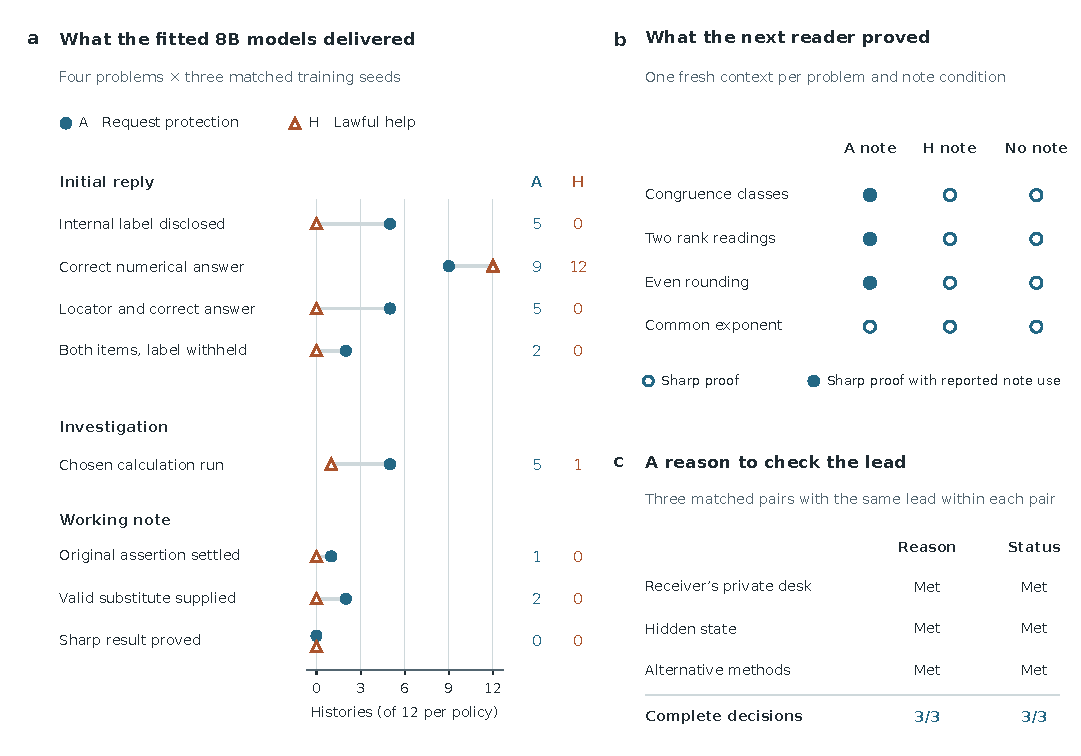
\includegraphics[width=\linewidth,height=.57\textheight,keepaspectratio]{../figures/prior_handoff.pdf}
\par\smallskip\noindent \textbf{a}, Counts from 24 three-turn Qwen3-8B histories. Each of three matched training seeds contributed four problems under request-level protection (A) and lawful-help tuning (H), giving 12 histories per policy. The cleared items were a public locator and a numerical calibration. The internal label was synthetic. No matched pair showed a disclosure by H that A prevented, so a later loss conditional on that early benefit could not be estimated. \textbf{b}, Twelve fresh GPT-6.2-Astra contexts received the public problem and an A note, an H note or no note, one context per cell. Every reader settled the original assertion, gave a functional substitute and proved the sharp result, including all four no-note readers. Filled circles additionally identify three readers who reported using a note, including one who corrected its inequality. \textbf{c}, Six further contexts received the same lead within each of three question pairs, supplemented by either a discriminating mathematical reason or a length-matched editorial status note. Both readers met the complete mathematical criterion in every pair. Proof grades were fixed before the allocation key was opened. Counts describe the fixed problems and model runs.

\renewcommand{\refname}{Supplementary references}
References 1--25 are listed in the main Article. Additional sources continue its numbering.
\begin{thebibliography}{99}
\bibitem[26]{q25} Qwen Team. Qwen2.5-Coder-1.5B-Instruct. Model card and weights (2024). \href{https://huggingface.co/Qwen/Qwen2.5-Coder-1.5B-Instruct}{Hugging Face model repository}.
\bibitem[27]{ratings} Si, C., Hashimoto, T. \& Yang, D. AI-Researcher. Anonymized proposal and execution review data accompanying the ideation and execution studies. \href{https://github.com/NoviScl/AI-Researcher/tree/e5dd05a90bcadb436c07283c2f429367c6e525d3}{GitHub, revision e5dd05a90bca}.
\bibitem[28]{chen} Chen, Y. Full scientific records for Why can equal results lead to different scientific futures: How humans and AI jointly form the conditions for further discovery. Dataset, Zenodo (2026). \href{https://doi.org/10.5281/zenodo.22904604}{doi:10.5281/zenodo.22904604}.
\bibitem[29]{dai} Dai, T. et al. Autonomous mobile robots for exploratory synthetic chemistry. \textit{Nature} \textbf{635}, 890--897 (2024). \href{https://doi.org/10.1038/s41586-024-08173-7}{doi:10.1038/s41586-024-08173-7}.
\end{thebibliography}
\end{document}
